%! Sample Fabrication
\subsubsection*{Sample Fabrication}
For all following depositions, the laser entrance window was cleaned before each process.
A pure \cro\ target was used for deposition of thin films on $5\times\qty{5}{\mm\squared}$ sapphire substrates in the four aforementioned orientations.
A first series of samples was produced by only varying the pulse number to achieve a series of thin films with varying thickness but constant laser fluence during deposition.
Therefore, the influence of thickness and growth rate can be deconvoluted.
% This is necessary, because the series of thicknesses that was achieved in the prior experiments was correlated to a series of growth rates.
The pulse energy was set to \qty{650}{\milli\joule} and the lens position to \qty{-2}{\cm}, resulting in a laser spot size of \qty{8}{\mm\squared}.
As described in section \ref{Sec:Methods_pld}, the laser pulse energy inside the PLD chamber is significantly lower than \qty{650}{\milli\joule}, due to absorption at the mirror, UV lens and laser entrance window.
By accounting for this attenuation, the resulting fluence on the PLD target is approx.\ \qty{2}{\joule\per\cm\squared}.
This corresponds to the standard configuration during all previous processes (pink square in Fig.\,\ref{Fig:Methods_fluence}).
This was repeated for three other lens positions, namely \qtylist{0;1;2}{\cm}, resulting in lower fluences of \qtylist{1.1;0.8;0.6}{\J\per\cm\squared}, respectively.
In Fig.\,\ref{Fig:Methods_fluence}, the yellow circles represent the probed laser fluences.
This set of samples is referred to as the 1st batch and is listed in Tab.\,\ref{Tab:Results_3_batch1}.
The laser spot sizes for different lens positions are depicted in Fig.\,\ref{Fig:Results_3_laserSpotSize}.

\begin{figure}
    \centering
    \includegraphics{laserSpotSize}
    \caption{
        Laser spot size $A$ depending on the lens position $L$: measured data (black) and fit according to $A(L)=a_2L^2+a_1L+a_0$ (red dashed).
        The fit parameters $a_2$, $a_1$ and $a_0$ are \qty{0.74}{\mm\squared\per\cm\squared}, \qty{5.3}{\mm\squared\per\cm} and \qty{15.6}{\mm\squared}, respectively.
    }
    \label{Fig:Results_3_laserSpotSize}
\end{figure}
\begin{figure}
    \centering
    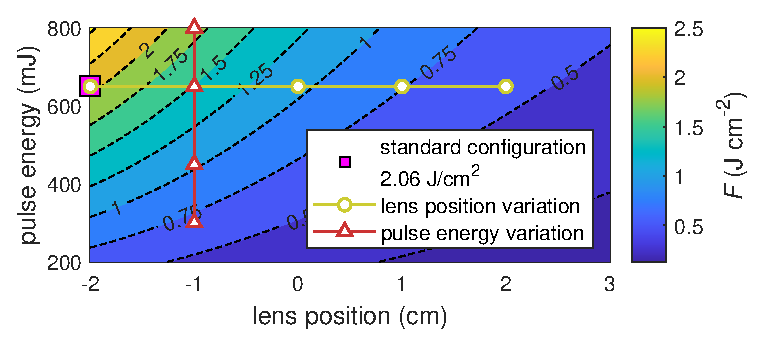
\includegraphics{fluence.eps}
    \caption{Laser energy density depending on the applied pulse energy and lens position. Smaller lens positions yield smaller spot sizes. A value of \qty{-2}{\cm} corresponds to the lens being as close as possible to the laser entrance window in the setup used for this work.
    The default configuration of \qty{650}{\milli\joule} and \qty{-2}{cm} yields typical fluences of about \qty{2}{\J\per\square\cm}.
    The triangles and circles represent the variation of laser fluence in this work, achieved by varying the pulse energy and lens position, respectively.}
    \label{Fig:Methods_fluence}
\end{figure}
\begin{table}
    \centering
    \caption{
        Processes of the first and second batch.
        For the first batch, a constant laser pulse energy of \qty{650}{\milli\J} was applied.
        The second batch was obtained by fixing the laser spot size to \qty{10}{\mm\squared}.
        For every process, \cro\ was deposited on four sapphire substrates with different orientations of \textit{c}-, \textit{r}-, \textit{m}- and \textit{a}-plane.
    }
    \begin{tabular}{lSSSSSS}
        \toprule
        
        & {$L$ (\unit{\cm})}
        & {$E_\mathrm{L}$ (\unit{\milli\J})}
        & {$A$ (\unit{\mm\squared})}
        & {$F$ (\unit{\J\per\cm\squared})}
        & {pulses (1k)}
        & {$t$ (\unit{\nm})}\\
        \midrule
        \parbox[t]{3mm}{\multirow{11}{*}{\rotatebox[origin=c]{90}{Batch 1}}}
        &-2      &  650      &   8       &   2.1       &   5       &   25  \\
        &        &           &           &           &   10      &   45  \\
        &        &           &           &           &   20      &   80  \\
        &        &           &           &           &   40      &   170  \\
        &        &           &           &           &   70      &   210  \\ \cmidrule{2-7}
        &0       &           &   16      &   1.1       &   8       &   40  \\
        &        &           &           &           &   20      &   90  \\
        &        &           &           &           &   35      &   40  \\ \cmidrule{2-7}
        &1       &           &   22      &   0.8     &   20      &   50  \\
        &        &           &           &           &   40      &   65  \\ \cmidrule{2-7}
        &2       &           &   29      &   0.6     &   17      &   30
        \\
        \midrule
        \parbox[t]{3mm}{\multirow{6}{*}{\rotatebox[origin=c]{90}{Batch 2}}}
        &-1      &  300      &   10       &   0.7       &   40       &   90  \\
        &        &  300      &            &   0.7       &   70       &   150  \\ \cmidrule{3-7}
        &        &  450      &            &   1.0       &   40       &   150  \\
        &        &  450      &            &   1.0       &   50       &   150  \\ \cmidrule{3-7}
        &        &  650      &            &   1.5       &   40       &   200  \\ \cmidrule{3-7}
        &        &  800      &            &   1.8       &   35       &   170  \\
        \bottomrule


    \end{tabular}
    \label{Tab:Results_3_batch1}
\end{table}

To investigate the influence of fluence independent of ablation area, a 2nd batch of samples was fabricated with a laser spot size of aprox.\ \qty{10}{\mm\squared} ($L=\qty{-1}{\cm}$) but varying laser pulse energy:
\qtylist{300;450;650;800}{\milli\joule}.
The achieved fluences are \qtylist{0.7;1.0;1.5;1.8}{\J\per\cm\squared} (red triangles in Fig.\,\ref{Fig:Methods_fluence}).
The pulse number was adjusted to achieve approximately the same thickness for all samples even though the growth rate vastly differs.
But note that for the different samples, the thickness is distributed from \qtyrange{100}{200}{\nm}.
Better results could be achieved in future experiments by first calibrating the growth rates for different fluences, and then adjusting the pulse numbers accordingly.
The process parameters of those samples are listed in Tab.\,\ref{Tab:Results_3_batch1}.

%! Measurements
\subsubsection*{Measurements}
For all samples, \thetaomega-scans as well as \textomega-scans were performed.
The symmetric reflections probed by the latter were (00.6), (02.4), (30.0) and (22.0) for \textit{c}-, \textit{r}-, \textit{m}- and \textit{a}-plane, respectively.
For \textit{r}- and \textit{a}-plane samples, the higher order reflection was chosen because the distance between the \cro\ peak and the \alo\ peak caused by \ce{W}-L\textalpha\textsubscript{1} radiation increases with higher angles.
Because both peaks are located at similar angles, this approach reduces the contribution of the substrate to the thin film Rocking curves.
% The thickness of all samples was determined by spectroscopic ellipsometry measurements.
To obtain more information about the relation between in-plane and out-of-plane lattice constants, \glspl{RSM} were performed on selected samples.
For every orientation, lattice planes have been chosen that have both a rather small tilt and high intensity:

\paragraph{\textit{c}-plane}
    For \textit{c}-plane samples, the thickness series grown at $L=\qty{-2}{\cm}$ and therefore a laser spot size of \qty{8}{\mm\squared} ($F=\qty{2.1}{\J\per\cm\squared}$) of the 1st batch was investigated.
    The asymmetric reflection that was used for probing the relaxation process is (02.10), which has an inclination angle of approx.\ \qty{32}{\degree} with respect to the sample surface.
\paragraph{\textit{r}-plane}
    All \textit{r}-plane samples fabricated in the 2nd batch with different laser pulse energies were investigated with \glspl{RSM}.
    For each sample, the $x$-axis of the sample -- containing the projection of the \textit{c}-axis -- is found by performing a \textphi-scan on the (03.0) reflection:
    This set of lattice planes has an inclination with respect to the surface, so the position of the peak in the diffraction pattern of the \textphi-scan reveals the $x$-axis.
    In this azimuth, an \gls{RSM} is recorded around the asymmetric (03.0) reflection and the symmetric (02.4) reflection.
    By rotating $\Delta\phi=\qty{90}{\degree}$, the $y$-axis lays in the scattering plane and another \gls{RSM} is performed around the symmetric (02.4) reflection.
    The twofold measurement of the symmetric reflection is necessary to calculate a possible lattice plane tilt for both $x$- and $y$-direction.
    % Note that no shear is calculated due to the asymmetric nature of the (03.0) reflection with respect to the \textit{r}-orientation\footnote{
        % For \textit{m}- and \textit{a}-plane rhombohedral structures, the crystal is symmetric under the transformation $\phi\rightarrow\phi+\qty{180}{\degree}$, which is not the case for \textit{r}-plane.
    % }.
    After performing the various corrections described in \ref{Sec:Methods_RSM}, the tilt angles can be calculated for both azimuths by
    \begin{eqnarray}
        \theta = \arccos\left(
            \frac{q_\perp}{|\mathbf{q}|}
        \right) \cdot\mathrm{sgn}\left(q_\parallel\right)\,,
        \label{Equ:Results_3_tiltAngle}
    \end{eqnarray}
    with $q_\perp$ and $q_\parallel$ being the \gls{oop}\ and \gls{ip}\ components of the scattering vector $\mathbf{q}$, respectively.
    The \gls{ip}\ and \gls{oop}\ strains are determined by comparing the observed (03.0) scattering vector to the scattering vector calculated from \cro\ bulk lattice constants:
    \begin{equation}
        \mathbf{q}_\mathrm{(03.0)} = 
        \left|\mathbf{q}_\mathrm{(03.0)}\right|\cdot
        \begin{pmatrix}
            \cos\alpha_{(03.0)|r}\\
            \sin\alpha_{(03.0)|r}
        \end{pmatrix}\,,
    \end{equation}
    with $|\mathbf{q}_{(03.0)}|$ calculated from \eqref{Equ:Methods_qAbs} and \eqref{Equ:Methods_dhkl}.
    $\alpha_{(03.0)|r}$ denotes the angle between the (03.0) reflection and the normal of the \textit{r}-planes; it can be calculated from \eqref{Equ:Methods_angleWRTc}:
    \begin{equation}
        \alpha_{(03.0)|r}
        = \qty{90}{\degree}-\left(
            \alpha_{(03.0)|c}-\alpha_{(01.2)|c}
        \right)
        = \alpha_{(01.2)|c}
        = \qty{57.62}{\degree}\,.
    \end{equation}
\paragraph{\textit{m}-plane}
    Similar to the \textit{r}-plane samples, all \textit{m}-plane samples from the 2nd batch were investigated.
    The samples were aligned to the $x$-axis by performing a \textphi-scan on the asymmetric (30.6) reflection, and an \gls{RSM} was recorded afterwards.
    By rotating $\Delta\phi=\qty{180}{\degree}$ while maintaining $2\theta$ and $\omega$, the scattering condition for $(30.\overline{6})$ is probed and an \gls{RSM} was recorded.
    The symmetric reflection (30.0) was also measured in this azimuth.
    The tilt angle and shear angle can be calculated according to \eqref{Equ:Results_3_tiltAngle} and \eqref{Equ:Methods_shearAngle}, respectively.
    As described in further detail in appendix \ref{Sec:App_Calc_mPlane}, the lattice constants can be calculated from the components of the scattering vectors:
    \begin{align}
        a_\perp &= \frac{\sqrt{12}}{q_\perp^{(30.\pm6)}} \,,\\
        a_\perp &= \frac{\sqrt{12}}{q_\perp^{(03.0)}}\,,\\
        c &= \frac{6}{q_\parallel^{(30.\pm6)}} \,.
    \end{align}
    $a_\perp$ denotes the $a$ lattice constant in direction of the normal to the sample surface.
    By rotating $\Delta\phi=\qty{90}{\degree}$, the \textit{y}-axis can be probed via asymmetric reflections $(\overline{4}2.0)$ and (22.0), which differ in the azimuth by $\Delta\phi=\qty{180}{\degree}$.
    A second symmetric reflection (30.0) is recorded in this azimuth.
    Similar to the $x$-axis, the tilt and shear angles, as well as the lattice constants can be calculated:
    \begin{align}
        (4\overline{2}.0):&\quad
            a_\perp = \frac{\sqrt{12}}{q_\perp^{(4\overline{2}.0)}}
            \quad,\quad
            a_\parallel = \frac{2}{q_\parallel^{(4\overline{2}.0)}}\,,\\
        (22.0):&\quad
            a_\perp = \frac{\sqrt{12}}{q_\perp^{(22.0)}}
            \quad,\quad
            a_\parallel = \frac{2}{q_\parallel^{(22.0)}}\,,\\
        (30.0):&\quad
            a_\perp = \frac{\sqrt{12}}{q_\perp^{(03.0)}}\,.
    \end{align}
    $a_\parallel$ denotes the $a$ lattice constant parallel to the $y$-axis.
    For detailed calculations of the former equations, see\ \ref{Sec:App_Calc_mPlane}.
    Note that all 6 measured reflections yield a value for $a_\perp$, and 2 measured reflections each yield 2 values for $c$ and $a_\parallel$, respectively.
    Therefore, for each lattice constant, the mean value is evaluated and the error is estimated by the standard deviation (cf.\ Fig.\,\ref{Fig:Results_3_pulse_ma_strainTilt}a).
\paragraph{\textit{a}-plane}
    All \textit{a}-plane samples from the 2nd batch were investigated and the method is similar to the one applied to the \textit{m}-plane samples.
    The azimuth of the \textit{x}-axis is found by performing a \textphi-scan on the (22.6) reflection, which also served for an \gls{RSM}.
    Rotating by $\Delta\phi=\qty{180}{\degree}$ yields the $(22.\overline{6})$ reflection and (22.0) is also measured.
    Similar to above, the sample is rotated by \qty{90}{\degree} to align to the $y$-axis and two more asymmetric reflections are recorded: (30.0) and (03.0).
    A second \gls{RSM} of (22.0) is also performed.
    This yields the following lattice constants for the $x$-axis:
    \begin{align}
        a_\perp &= \frac{4}{q_\perp^{(22.\pm6)}} \,,\\
        a_\perp &= \frac{4}{q_\perp^{(22.0)}}\,,\\
        c &= \frac{6}{q_\parallel^{(22.\pm6)}} \,,
    \end{align}
    and for the $y$-axis:
    \begin{align}
        (30.0):&\quad
            a_\perp = \frac{3}{q_\perp^{(30.0)}}
            \quad,\quad
            a_\parallel = \frac{3}{\sqrt{3}q_\parallel^{(30.0)}}\,,\\
        (03.0):&\quad
            a_\perp = \frac{3}{q_\perp^{(03.0)}}
            \quad,\quad
            a_\parallel = \frac{3}{\sqrt{3}q_\parallel^{(03.0)}}\,,\\
        (22.0):&\quad
            a_\perp = \frac{4}{q_\perp^{(22.0)}}\,.
    \end{align}
    For detailed calculations, see\ \ref{Sec:App_Calc_aPlane}.
    Again, for the lattice constants obtained from several reflections, the mean and standard deviation are calculated (cf.\ Fig.\,\ref{Fig:Results_3_pulse_ma_strainTilt}b).
